\documentclass[a4paper]{jsarticle}
\usepackage[dvipdfmx, hiresbb]{graphicx}
\usepackage{booktabs}
\usepackage{macros}

\newcommand{\Sh}{\mathbf{Sh}}
\newcommand{\PSh}{\mathbf{PSh}}
\newcommand{\ftorSh}{\mathit{Sh}}
\newcommand{\ftorFgt}{\mathit{Fgt}}
\newcommand{\Cov}{\operatorname{Cov}}

\begin{document}
\title{ゼミノート \#2 \\ Sites and Sheaves}
\author{七条彰紀}
\maketitle

\section{Motivation.}
scheme, stack等には以下のような包含関係がある.
\[\xymatrix{
    {} & \text{Algebraic Stack} \ar@{^{(}->}[r]& \text{Stack} \ar@{^{(}->}[r]& \text{Presheaf of Grupoids} \\
    \text{Scheme} \ar@{^{(}->}[r]\ar@{^{(}->}[ru]& \text{Algebraic Space} \ar@{^{(}->}[r]\ar@{^{(}->}[u]&
        \text{Space} \ar@{^{(}->}[r]\ar@{^{(}->}[u]& \text{Presheaf of Sets} \ar@{^{(}->}[u]
}\]
最終的にセミナーを通じて我々が定義したいのはalgebraic stackであるが,
今回はそれよりも定義が簡素な``space"を定義する.
先にspaceの定義文を示そう.

\begin{Def}[Space, \cite{GomezAS} p.26]
    $S$ :: schemeとする.
    Space over $S$ (or $S$-space)とは,
    big etale site over $S$上にある,集合のsheafである.
\end{Def}
ここに現れる``big etale site"と``big etale site上のsheaf"を以下で定義する.
さらにsheafの射について幾つか定義をすれば,
algebraic spaceまで定義できる.

定義だけではspaceのlocalは性質を調べる手段がないため,
次回は「高次版のsheafの貼り合わせ」と呼べる``Descent theory"を学ぶ.

\section{Definitions : Sites.}
以下で導入するGrothendieck topologyは,
「Sheafを定義するのに必要な位相空間の定義を抽出し,圏論的に一般化したもの」である.
$X$ :: toplological spaceとし,sheaf on $X$の定義を見なおしてみよう.
すると,sheaf on  $X$は次に挙げるもののみを用いて定義されていると分かる.
\begin{enumerate}
    \item $X$の開部分集合と包含写像が成す圏.
    \item 開部分集合$U \subseteq X$のopen covering.
    \item 同じく$U$のopen covering :: $\{U_i\}_i$が与えられたときの族$\{ U_i \cap U_j \}_{i,j}$
\end{enumerate}
そこで次のように定義する.

\begin{Def}[Grothendieck Topology]
    $\cat{C}$ :: cateogoryについて,
    $\cat{C}$上のGrohendieck topologyは
    任意の$X \in \cat{C}$に
    $\cat{C}$の射の集まり(collection)$\{X_i \to X\}_{i \in I}$を対応させる$\Cov$で構成される.
    さらに,$\Cov$は以下を満たすように要請される.
    \begin{enumerate}[label=(\alph*)]
        \item
            $X' \to X$ :: isoならば$\{X' \to X\} \in \Cov(X)$.
        \item
            $\{U_i \to U\} \in \Cov(U), V \to U \in \cat{C}$について,
            $\{U_i \times_U V \to V\} \in \Cov(V)$.
        \item
            $\{U_i \to U\}_i \in \Cov(U)$をとり,
            さらに各$i$について$\{V_{i,j} \to U_i\}_j \in \Cov(U_i)$をとる. \mbox{}\\
            この時,合成も$\Cov$に入っている : $\{V_{i,j} \to U_i \to U\}_{i,j} \in \Cov(U)$.
    \end{enumerate}
\end{Def}

\begin{Remark}\label{rem:grotop_stablecond}
    $\Cov$の条件のうち,
    (b), (c)はそれぞれstable under base change, stable under compositionに対応する.
\end{Remark}

$\Cov$の元には大抵,以下の条件が課される.
\begin{Def}[(Jointly) Surjective Family]
    ある圏の射の集まり$\{U_i \to U\}_i$について,
    \[ \bigsqcup_i U_i \to U \]がsurjectiveである時,
    (同値な条件として,
    $\im (U_i \to U)$のset-theoritic unionが$U$に等しい時,)
    この集まり$\{U_i \to U\}$を(jointly) surjective familyという.
\end{Def}

\begin{Remark}
    ここで「集合」ではなく「集まり」という言葉を用いたのは,
    これらが集合ではない可能性があるからである.
\end{Remark}

\begin{Def}[Site]
    圏$\cat{C}$と$\cat{C}$上のGrothendieck topology :: $\Cov$の組をsiteと呼ぶ.
    siteに対し,その部分である圏をthe underlying categoryと呼ぶ.
    しばしば$\Cov$を略して$\cat{C}$のみでsiteを表す.
\end{Def}

\begin{Def}[Localized Site.]
    site :: $\cat{C}$と$X \in \cat{C}$について,
    localized site :: $\cat{C}/X$を以下のように定義する.

    $\cat{C}/X$のunderlying categoryはslice cageory :: $\cat{C}/X$である.
    したがって対象は$\cat{C}$内の$X$への射である.
    Grothendieck topology :: $\Cov$は,
    \[
        \{ [U_i \to X] \to [U \to X] \}_i \in \Cov([U \to X])
        \implies \{U_i \to U\} \in \Cov(U).
    \]
    のように定められる.
\end{Def}

\begin{Def}[Diagrams (or Comma Site).]
    $\Delta$ :: category, $\cat{C}$ :: site, 
    $F \colon \Delta^{op} \to \cat{C}$ :: functorとする.
    この時site :: $\cat{C}_F$を以下のように定める.

    まずundrelying categoryは$(\id[\cat{C}] \downarrow F)$である.
    したがって対象は$X \to F(\delta) \ (\delta \in \Delta)$である.
    $\Cov$は以下のように定める.
    \[
        \left\{
        \xymatrix@R=8pt{
            X'_i \ar[d]\ar[r]^-{f_i^{\flat}}& X \ar[d]\\
            F(\delta_i) \ar[r]_-{f_i}& F(\delta)
        }
        \right\} \in \Cov([X \to F(\delta)])
        \implies
        f_i \colon \delta \to \delta_i \text{ :: iso. and }
        \{f_i^{\flat} \colon X'_i \to X \} \in \Cov(X).
    \]
\end{Def}

\begin{Def}[Continuous Functor.]
    $\cat{C}, \cat{C}'$ :: sites, 
    $T (T')$ :: topos associated $\cat{C} (\cat{C}')$とする.
    $f \colon \cat{C} \to \cat{C}'$ :: functorがcontinuousとは,
    以下の$2$つが成立すること:
    \begin{enumerate}
        \item 
        任意の$X \in \cat{C}$と$\{U_i \to X\}_i \in \Cov_{\cat{C}}(X)$について,
        \[ \{ f(U_i) \to f(X) \}_i \in \Cov_{\cat{C}'}(f(X)) \]となる.

        \item
        $\cat{C}$の任意の射$X_1 \to Y, X_2 \to Y$について,
        fiber product :: $X_1 \times_Y X_2$が$\cat{C}$に存在するならば,
        \[ f(X_1 \times_Y X_2) \iso f(X_1) \times_{f(Y)} f(X_2). \]
    \end{enumerate}
\end{Def}

\begin{Remark}    
    $X, X'$ :: topological spaceについて,
    $O(X), O(X')$ :: classical site,
    $f \colon X \to X'$ ::continuous mapとする.
    この時,$f^{-1} \colon O(X') \to O(X)$ :: continuous functor.
    2つめの条件は$f^{-1}$が$\cap$と交換することと対応する.
\end{Remark}

\begin{Remark}
    後に示すように,
    continuous functorはよくあるケースでcategory of sheaves on siteの間の関手を誘導する.
    これはschemeの間のcontinuous mapが
    category of sheaves on schemeの間の
    関手(e.g. inverse image functor, direct image functor)を定めるのと同じである.
\end{Remark}

\section{Examples : Sites.}

\subsection{Site.}
\begin{Example}[Classical topology.]
    $X$ :: topological spaceとし,
    $O(X)$を以下のような圏とする.
    \begin{description}[labelindent=5mm]
        \item[対象] $X$の開集合.
        \item[射] 包含射.
    \end{description}
    この時,$U \in O(X)$のcovering :: $\Cov(U)$を,
    $U$への包含射のみから成るjointly surjective familyの集合
    \footnote{ 包含射の個数は高々$2^{\#X}$以下の濃度なので,familyの集まりは集合. }
    とする.

    以上で定まるsite :: $(O(X), \Cov)$は
    通常のtopologyをGrothendieck topologyの枠組の中で再現している.
\end{Example}

以下で主に用いるのは,
$\cat{C}$がslice category :: $\Sch/X \ (X \in \Sch)$の部分圏であるようなsiteである.
$X \in \Sch$に対して,
このようなsiteはunderlying category ($\subset \Sch/X$)と
Grothendieck topology ($\Cov$)からなるから, 
以下の図の(a) $U \to X$, (b) $U_i \to U$がどのようなものであるか定めれば定義できる.
\begin{center}
     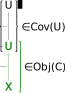
\includegraphics[width=5cm]{./images/site.pdf}
\end{center}
すなわち,以下の未完成な定義文をテンプレートとする,一連の定義文の群がある.
\begin{Def}[$***$ site]
    $X$ :: schemeについて,
    圏$\cat{C}$を以下で定める.
    \begin{description}[labelindent=5mm]
        \item[対象] (a)である射$U \to X$.
        \item[射]   二つの対象の間の射$[U \to X] \to [U' \to X]$は,$X$-morphism :: $U \to U'$.
    \end{description}
    $[U \to X] \in \cat{C}$に対して,
    $\Cov(U)$を(b)である射の集まり$\{U_i \to U\}_i$であって
    jointly surjective familyであるものの集まりとする.

    以上の$\cat{C}$と$\Cov$からなるsiteを $***$ site of $X$と呼ぶ.
\end{Def}

注意(\ref{rem:grotop_stablecond})で触れたとおり,
性質(b)がstable under base change \& compositionであれば,
以上のテンプレートはsiteの定義文と成る.

\begin{samepage}
\begin{Def}
    以上の定義文テンプレートを用いて,(a), (b)と各siteの定義を以下のように対応させる.
    (a)が``--"とある箇所は「$\Sch/X$の任意の射」を意味する.
    さらに,``open inclusion"はZariski開集合の間にある包含射のことである
    (したがってsmall Zariski siteのunderlying categoryにはZariski開集合しか無い).

\begin{table}[ht]
\begin{tabular}{c|lllllll}
\toprule
    $***$ & small Zariski  & big Zariski    & small etale & big etale\\ \midrule
    (a)   & open immersion & --             & etale       & --       \\
    (b)   & open immersion & open immersion& etale       & etale    \\ \hline \hline
    $***$ & lisse-etale & smooth & fppf                                   & fpqc                  \\ \midrule
    (a)   & smooth      & smooth & --                                     & --                    \\
    (b)   & etale       & smooth & flat\&locally of finite presentation & flat\&quasi-compact \\ \bottomrule
\end{tabular}
\end{table}

    図の再掲:
    \begin{center}
         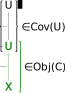
\includegraphics[width=5cm]{./images/site.pdf}
    \end{center}
\end{Def}
\end{samepage}

\begin{Remark}
``fppf"は
``fid\`{e}lement plate de pr\'{e}sentation finie"(仏語)すなわち
``faithfully flat and of finite presentation"の略である.
flat\& locally of finite presentationならば実際にこのように成る.
同様に``fpqc"は``fid\`{e}lement plat et quasi-compact"(仏語)すなわち
``faithfully flat and quasi-compact"の略である.
\end{Remark}

\begin{Def}
    $***$ site of $X$の記号を以下のように定める.
\begin{table}[ht]
\begin{tabular}{c|lllllllll@{}}
    \toprule
    $***$ & small Zariski     & big Zariski       & small etale      & big etale\\ \midrule
    名前    & $\mathrm{Zar}(X)$ & $\mathrm{ZAR}(X)$ & $\mathrm{Et}(X)$ & $\mathrm{ET}(X)$ \\ \hline \hline
    $***$ & lisse-etale         & smooth           & fppf               & fpqc               \\ \midrule
    名前    & $\mathrm{Lis\mdash Et}(X)$ & $\mathrm{Sm}(X)$ & $\mathrm{Fppf}(X)$ & $\mathrm{Fpqc}(X)$ \\ \bottomrule
\end{tabular}
\end{table}

    \cite{StacksProj}ではbig Zariski site of $X$を$(\Sch/X)_{Zariski}$などと書く.
\end{Def}

\subsection{Point.}
以下はsmall/big etale siteのみで使われるものである.
\begin{Def}[Geometric Point, Etale Neighborhood, \cite{ASS} 1.3.15.]
\begin{myenum}{\roman*}
    \item 
    $X$ :: schemeに対し,
    $k$ :: separabely closed fieldを用いて
    $\bar{x} \colon \Spec k \to X$と表される射をgeometric pointと呼ぶ.

    \item
    geometric point :: $\bar{x} \colon \Spec k \to X$について,
    $\bar{x}$のetale neighborhoodとは
    $U \to X$がetaleであるような以下の可換図式のことである.
    \[\xymatrix{
        {} & U \ar[d]\\
        \Spec k \ar[r]_-{\bar{x}} \ar[ru]& X
    }\]

    \item
    geometric point :: $\bar{x} \colon \Spec k \to X$について,
    $\bar{x}$の$2$つのetale neighborhood :: $U_1, U_2$を考える.
    この時,$U_1$と$U_2$の間の射とは,
    以下の図式を可換にするmorphism of schemes :: $\eta \colon U_1 \to U_2$のことである.
    \begin{equation*}
    \begin{xy}
        (0,17.32) *{U_1}="U1", (20, 17.32) *{U_2}="U2",
        (-20, 3) *{\Spec k}="k", (10,0) *{X}="X",
        \ar "U1";"X" \ar "U2";"X" \ar "U1";"U2"^{\eta}
        \ar "k";"U1" \ar "k";"U2" \ar "k";"X"
    \end{xy}
    \end{equation*}
\end{myenum}
\end{Def}

\begin{Remark}
    より一般的なpoint of siteの定義が存在する(\cite{StacksProj} Tag 04JU).
    これはetaleか否かに依らず採用できる.
    しかしこの一般的な定義は複雑であるし,
    我々はsmall/big etale siteしか扱わないので,
    我々は以上の定義のみ用いる.
\end{Remark}

\subsection{Continuous Functor.}
\begin{Example}
    inclusion $\mathrm{Zar}(X) \inclmap \mathrm{Et}(X) \inclmap \mathrm{Fppf}(X)$
\end{Example}
\begin{Example}
    flat morphism :: $f \colon X \to Y$をとり,
    $f$によるpullback functorを$P_{f}$とする.
\end{Example}

\section{Definitions : Sheaves.}
\begin{Def}[Sheaf, Topos, Morphism of Topoi.]
    \begin{myenum}{\roman*}
    \item
    site :: $S$上のpresheafとは,
    functor :: $\shF \colon S^{op} \to \Sets$のことである.

    \item
    presheaf on $S$ :: $\shF$がsheafであるとは,
    以下の図式がequalizer diagramであるということ.
    \[\xymatrix{
        \shF(U) \ar[r]& \prod_{i \in I} \shF(U_i)
            \ar@<1mm>[r]\ar@<-1mm>[r]& \prod_{(i,j) \in I \times I} \shF(U_i \times_U T_j)
    }\]
    ここで右の並行射は
    それぞれ射影$\pr_1(, \pr_2) \colon U_i \times U_j \to U_i(, U_j)$から
    $\shF$により誘導される射である.

    \item
    Site :: $S$上の,
    圏$\cat{C}(=\Sets, \mathrm{Rings}, \mathrm{AbGrp}, \dots)$への
    presheafの圏を$\PSh(S, \cat{C})$,sheafの圏を$\Sh(S, \cat{C})$と書く.

    \item
    morphism of shaeves :: $\shF \to \shF'$とは,
    natural transformationのことである.

    \item
    $T$ :: categoryがtoposであるとは,
    category of sheaves of sets on a siteと圏同値であるということである.

    \item
    $T, T'$ :: topoiとする.
    morphism of topoi :: $f \colon T \to T'$とは,
    以下の$3$つの射($2$ functor and $1$ isomorphism.)からなる.
    \[
        f_* \colon T \to T', \quad f^* \colon T' \to T,
        \quad \phi \colon \Hom_{T}(f^*(-), -) \isomap \Hom_{T'}(-. f_*(-)).
    \]
\end{myenum}
\end{Def}

\begin{Remark}
    上で定義したsheaf of setsと同様に,
    sheaf of abelian groups, sheaf of rings, ...が定義できる.
    これらはそれぞれsheaf of setsの圏 :: $\Sh(\cat{C}, \Sets)$における
    abelian group objects, ring objects, ...と定義される.
\end{Remark}

\begin{Remark}
    ``Topos"はギリシャ語で「場(place)」を意味する.
    ギリシャ語なので複数形は``topoi".

    $X$ :: schemeについて,
    $X$に関するtoposを$X_{et}, X_{ET}, \dots$などと書く.
    著者(例えば\cite{StacksProj})によっては
    これらの記号を$\Sch/X$をunderlying catgoryとするsiteに用いる.
    しかし``Grothendieck’s insight is that the basic object of study is the topos, not the site."
    (M.Olsson ``Stacks")というということから,
    toposにsiteより簡単な記号を与えるのは理解できることである.
\end{Remark}

\begin{Def}[Ringed Topos.]
\begin{myenum}{\roman*}
    \item
    $T$ :: toposと$T$のring object :: $\Lambda$を合わせてringed toposと呼ぶ.

    \item
    morphism of ringed topoi :: $(f, f^{\#}) \colon (T, \Lambda) \to (T', \Lambda')$は,
    \begin{itemize}
        \item morphism of topoi :: $f=(f_*, f^*, \phi) \colon T \to T'$と,
        \item morphism of ring in $T'$ :: $f^{\#} \colon \Lambda' \to f_* \Lambda$
    \end{itemize}
    の組である.
\end{myenum}
\end{Def}

\begin{Def}[Stalk, \cite{ASS} 1.3.15.]
    $U \in I_{\bar{x}}$について,$\shF(U)$から$\shF_{\bar{x}}$への標準的射がある.
    この射による$s \in \shF(U)$の像を$s_{\bar{x}}$と表し,
    germ of $s$ at $\bar{x}$と呼ぶ.
\end{Def}

\section{Examples : Sheaves.}
\begin{Example}
    $X$ :: schemeと,
    $\Sch/X$の部分圏をunderlying categoryとするsite :: $\cat{C}$(e.g. small/big Zariski site)について,
    $\ftor{X}(-)=\Hom_{\cat{C}}(-, X)$で
    functor :: $\ftor{X} \colon \cat{C} \to \Sets$を定める.
    この時,$\ftor{X}$ :: presheaf on $\cat{C}$.
    特にsmall/big Zariski site, small/big etale siteではsheafである.
\end{Example}

\begin{Example}
    constant (pre)sheaf
\end{Example}

\section{Propositions : Sheaves.}
\begin{Thm}
    $\cat{C}$ :: siteとする.
    忘却関手
    \[
        \ftorFgt \colon
        \text{(Category of Sheaves on $\cat{C}$)}
            \to \text{(Category of Presheaves on $\cat{C}$)}.
    \]
    はleft adjoint functor :: $\ftorSh$を持つ.
\end{Thm}

\begin{Prop}
\cite{ASS} 1.4.9
$\ftor{X}$ :: sheaf.
\end{Prop}

\section{Definitions : Morphism of Shaves.}
\begin{Def}[Injective, Surjective]
\end{Def}

\section{Examples : Morphism of Shaves.}

\section{Propositions : Morphism of Shaves.}
\begin{Prop}
    inj/surj/iso at stalk.
\end{Prop}
\bibliographystyle{jplain}
\bibliography{reference}
\end{document}
